\subsection{JAM based on Surface Brightness} \label{sec:results_JAM_SB}

\paragraph{... with the Lens Mass Model.} Our first JAM model uses the mass distribution which we found from lensing constraints in Section \ref{sec:results_lensing} to generate an independent prediction for the $v_\text{rms}$ curve following the procedure in Section \ref{sec:model_JAM}. In addition to the flat rotation curve model with $\alpha = 1$ in Table \ref{tab:bestfitlensmodel}, we also investigate a lens model, which was found as a best fit to the lensing images when assuming a [TO DO: rising or droppint???] rotation curve slope of $\alpha=1.1$. The predictions are compared with the data in Figure \ref{fig:JAM_modelL}. The agreement between the lensing prediction and the observed kinematics within $R' \sim 3$ arcsec is striking, especially around the Einstein radius. The $\alpha = 1$ model fits the wings nicely, while the $\alpha = 1.1$ model recreates almost exactly the observed central dip. The sharp drop in $v_\text{rms}$ around $R' \sim 3$ arcsec cannot be reproduced, however. But outside of the Einstein radius our lensing models are only extrapolations and the true constraint is around the Einstein radius.

%==================================================================

\begin{figure}
  \centering
  \includegraphics[height=6cm]{fig/lensing_JAM_comparision.ps}
  \caption{Comparison (not a fit!) of the symmetrized stellar $v_\text{rms}$ data of J1331 (blue dots) with JAM models generated from mass distributions which were independently derived from lensing constraints in Section \ref{sec:results_lensing}. The red solid line corresponds to the lens model for a flat rotation curve ($\alpha = 1$) in Table \ref{tab:bestfitlensmodel}; the green line is a best fit lens model found analogously from the image positions, but for a fixed rotation curve slope of $\alpha = 1.1$. For the JAM modelling a best fit MGE to the lens mass models were used, as well as the observed surface brightness MGE in Table \ref{tab:MGEF814W}, assuming velocity isotropy $\beta_z = 0$ and an inclination of $i = 70^\circ$.The red and black dotted lines are the Einstein radius and the effective half-light radius, respectively.}
  \label{fig:JAM_modelL}
\end{figure}

%==================================================================


\paragraph{... with "Mass-follows-Light" and Velocity Anisotropy.} Our second JAM model is a mass-follows-light model, which are often used in dynamical JAM modelling (e.g. \citet{GlennEC,Cap06}), where the mass distribution ins generated by multiplying the intrinsic light distribution $\nu(R,z)$ (the MGE given in Table \ref{tab:MGEF814W} deprojected according to the inclination) by a constant total mass-to-light ratio  $\Upsilon_\text{I,tot}^\text{dyn}$. This assumes that the dark matter is always a constant fraction of the total matter distribution everywhere. This simplified model sometimes gives good representations of the inner parts of galaxies, where the stellar component dominates. Testing this model for J1331 is also motivated by our findings from lensing in Section \ref{sec:results_lensing}, where around the Einstein radius total and luminous mass seem to have a similar distribution.
\\In addition to the free fit parameter  $\Upsilon_\text{I,tot}^\text{dyn}$, we also allow for a overall constant but non-zero velocity anisotropy $\beta_z$. The best fit is found by minimizing $\chi^2$ between the $v_\text{rms}$ data and model prediction and is demonstrated in Figure \ref{fig:JAM_modelA2}. For $\beta_z$ we impose the fitting limits $\beta_z \in [-0.5,+0.5]$. While the outer parts of galaxies often show radially biased velocity anisotropy up to $\sim 0.5$ (from dynamical modelling of observed elliptical galaxies (e.g. \citet{Kronawitter2000}) and cosmological simulations (e.g. \citet{2004MNRAS.352..535D,2001ApJ...557..533F}), the centers of galaxies are near-isotropic or have  negative velocity anisotropy \citep{2003ApJ...583...92G}. Only in extreme models (e.g. around in-spiralling supermassive black holes \citep{1997NewA....2..533Q}) velocity anisotropies as low as $\sim -1$ have been found. A lower limit of $\beta_z \geq -0.5$ is a realistic assumption for J1331, for which we do not expect extreme dynamical conditions. The best fit in Figure \ref{fig:JAM_modelA2} however strives to very negative velocity anisotropies to be able to get the deep central dip in the  $v_\text{rms}$ curve. But $\beta_z = -0.5$ is not even a remotely agreeable fit and lower anisotropies are not to be expected and realistic. We also tested radial profiles for $\beta_z(R)$ of the form proposed by \citet{BaesVanHese}, which was however equally unable to reproduce the data. We conclude, that this is due to the well-known degeneracy between anisotropy and mass profile [TO DO: REF] and the mass-follows-light model is \emph{not} a good representation of the mass distribution in J1331's inner regions.


%==================================================================

\begin{figure}
  \centering
  \includegraphics[height=6cm]{fig/jam_A2_vrms.ps}
  \caption{Comparison of the symmetrized $v_\text{rms}$ data of J1331 (blue dots) with a best fit dynamical JAM model (solid red line) assuming mass-follows-light and with two free parameters: $\Upsilon_\text{I,tot}^\text{dyn}$, the total I-band mass-to-light ratio found from dynamics, which converts the observed surface brightness in Table \ref{tab:MGEF814W} into a mass distribution, and the velocity anisotropy parameter $\beta_z$. The ``best'' fit is $\Upsilon_\text{I,tot}^\text{dyn} = 4.8 \pm 0.1$ and $\beta_z = -0.5$, where the latter is however pegged at the lower limit of the allowed value range. This is obviously not a good model.}
  \label{fig:JAM_modelA2}
\end{figure}

%==================================================================

\paragraph{... with Increasing Mass-to-Light Ratio.} In Section \ref{sec:results_lensing} we found from the lensing, that the light distribution might drop faster with radius than the mass distribution. This would correspond to a radially increasing total mass-to-light ratio. As velocity anisotropy alone cannot explain the observed kinematics in a simple a mass-follows-light model, we now allow for an mass-to-light ratio gradient in the JAM modelling to generate a mass model from the light distribution in Table \ref{tab:MGEF814W}. We do this by assigning each of the five Gaussians in the MGE its own total mass-to-light ratio $\Upsilon_{\text{I,tot,}i}$ and replace the total luminosity in Equation \ref{eq:centralItotalL} $L_i$ with the Gaussians total Mass $M_i = \Upsilon_{\text{I,tot,}i} L_i$. We treat the five $\Upsilon_{\text{I,tot,}i}$ as free parameters and only require that $\Upsilon_{\text{I,tot,}j} \geq \Upsilon_{\text{I,tot,}i}$ when the corresponding $\sigma_j \geq \sigma_i$ to ensure an overall mass-to-light ratio that is increasing with radius.
\\Figure \ref{fig:enclMass_modelG} shows the (local projected) mass-to-light ratio gradient generated by the best fit to the dynamics data, which rises from $\Upsilon_\text{I,tot} = 2.53$ in the center and approaches a value of $\Upsilon_\text{I,tot}$ outside of the fitted region at $R'\gtrsim 3$ arcsec of $\Upsilon_\text{tot} = 7.60)$. The central mass-to-light ratio corresponds to the Chabrier IMF stellar mass-to-light ratio found by [TO DO: REF: TREU ET AL 2011] $\Upsilon_\text{I,*}^\text{chab} = 2.5 \pm 0.6$ [TO DO: introduce and explain????]. The strong rise of $\Upsilon_\text{I,tot}(R')$ cannot be explained by an increase in the stellar $\Upsilon_\text{i,*}$ alone [TO DO: Really??? Maybe it would have dropped again in the blue disk, if I had allowed for it????], so we deduce that we might need  contribution of dark matter halo in J1331.
\\Figure \ref{fig:JAM_modelG} shows that the best fit model greatly reproduces the central dip in the $v_\text{rms}$ curve, even though it has slight problems fitting the drop around $R' \sim 4$ arcsec. The latter might be because we only allowed the $\Upsilon_\text{I,tot}(R')$ to rise. A slight drop could be expected when the reddish bulge turns into the bluish disk and the contribution of the stellar component becomes less due to a lower $\Upsilon_\text{I,*}$ for younger and bluer populations.
\\In Figure \ref{fig:enclMass_modelG} we overplot the enclosed mass profile with the Einstein mass $M_\text{ein} = (7.77 \pm 0.33) \cdot 10^{10} M_\odot$ at the Einstein radius found from lensing in Table [TO DO: REF]. The agreement between the Einstein mass and the independently found $M(<R_\text{ein}) = 7.49 \cdot 10^{10} M_\odot$ from dynamical modelling is striking.


%==================================================================

\begin{figure*}
\centering
\begin{subfigure}{.5\textwidth}
  \centering
  \includegraphics[height=6cm]{fig/jam_G_vrms.ps}
  \caption{Comparison of $v_\text{rms}$ data and best fit model.}
  \label{fig:JAM_modelG}
\end{subfigure}%
\begin{subfigure}{.5\textwidth}
  \centering
  \includegraphics[height=6cm]{fig/jam_G_enclMass.ps}
  \caption{Projected local mass-to-light ratio profile and enclosed mass.}
  \label{fig:enclMass_modelG}
\end{subfigure}
\caption{JAM model found by fitting an increasing total mass-to-light ratio $\Upsilon_\text{I,tot}(R')$ profile used to generate a mass model from the light distribution.  This is done by assigning a different mass-to-light ratio to each Gaussian in the MGE in Table \ref{tab:MGEF814W}. \emph{Panel (a):} Comparison between the stellar $v_\text{rms}$ data (blue points) and the best fit model (green line). \emph{Panel (b):} Enclosed mass inside the projected radius $R'$ on the sky (green line, right axis) and projected mass-to-light profile $\Upsilon_\text{I,tot}(R')$ along the major axis (blue line, left axis) of the best fit model. The enclosed mass curve is overplotted with the independent finding for the Einstein mass $\pm 4 \%$ in Table \ref{tab:bestfitlensmodel} (red dot) at the Einstein radius (red dotted line). The best fit mass-to-light ratios of the first four Gaussians are plotted against each Gaussians $\sigma$ (yellow stars). The two Gaussians with the largest $\sigma$ (the fifth is not shown) have the same best fit mass-to-light ratio. Overplotted is also the effective half-light ratio $R_\text{eff}$ (black dotted line).  [TO DO: These plots look slightly different, because they were created directly as ps files. The others have to be re plotted to look the same.] }
\label{fig:modelG}
\end{figure*}

%==================================================================